\documentclass[twoside]{article}


%\usepackage{hyperref}
\usepackage{amssymb,amsthm}
\usepackage{amsmath}
\usepackage{color}
\usepackage{ esint }
\usepackage{mathabx}
\usepackage{MnSymbol}
\usepackage{fancyhdr}
\usepackage{soul} 
%\usepackage{times}
\usepackage{tikz}
%\usepackage[latin1]{inputenc}

\usepackage{comment}
\usepackage{url}
\usepackage{xcolor}
\usepackage{adjustbox}
\usepackage{hyperref}

\newtheorem{thm}{Theorem}[section]
\newtheorem{cor}[thm]{Corollary}
\newtheorem{lem}[thm]{Lemma}

\newtheorem{defi}[thm]{Definition}
\newtheorem{prop}[thm]{Proposition}
\theoremstyle{remark}
\newtheorem{comentario}{Remark}
\newtheorem{ejemplo}{Example}


\makeatletter
\newcommand{\labitem}[2]{%
\def\@itemlabel{\textbf{#1}}
\item
\def\@currentlabel{#1}\label{#2}}
\makeatother




\title{A generalized Sitnikov problem with primary bodies in both homographic and rigid motions}
\author{Gast\'on Beltritti \thanks{SECyT-UNRC and CONICET}\\
Dpto. de Matem\'atica, Facultad de Ciencias Exactas Físico-Químicas y Naturales\\
Universidad Nacional de R\'{i}o Cuarto\
(5800) R\'{\i}o Cuarto, C\'ordoba, Argentina,\\
\url{gbeltritti@exa.unrc.edu.ar}\\[3mm]
Fernando D. Mazzone \thanks{SECyT-UNRC, FCEyN-UNLPam}\\
Dpto. de Matem\'atica, Facultad de Ciencias Exactas, F\'{\i}sico-Qu\'{\i}micas y Naturales\\
Universidad Nacional de R\'{i}o Cuarto\\
(5800) R\'{\i}o Cuarto, C\'ordoba, Argentina,\\
\url{fmazzone@exa.unrc.edu.ar}\\
Martina G. Oviedo \thanks{SECyT-UNRC, CIN}\\
Dpto. de Matem\'atica, Facultad de Ciencias Exactas, F\'{\i}sico-Qu\'{\i}micas y Naturales\\
Universidad Nacional de R\'{i}o Cuarto\\
(5800) R\'{\i}o Cuarto, C\'ordoba, Argentina,\\
\url{martinagoviedo@gmail.com}
}

\date{}


\newcommand{\rr}{\mathbb{R}}
\newcommand{\nn}{\mathbb{N}}


\newcounter{example}

\setcounter{example}{1}


\newenvironment{example}{\noindent\textit{Example} \arabic{example}.}{\addtocounter{example}{1}}




\begin{document}


\maketitle
%
% \begingroup%Locallizing the change to `thefootnote'.
%     \renewcommand{\thefootnote}{}%Removing the footnote symbol.
%     %
%     \footnotetext{%
%     %   2010 Mathematics Subject Classification
%     %   http://www.ams.org/msc/
%     \textbf{2010  AMS Subject Classification.} Primary: .
%     Secondary: .
%     }%
%         \footnotetext{%
%     \textbf{Keywords and phrases.}  .
%     }%
%     \endgroup
%
%
%
%

\begin{abstract}


\end{abstract}




\pagestyle{fancy} \headheight 35pt \fancyhead{} \fancyfoot{}

\fancyfoot[C]{\thepage} \fancyhead[CE]{\nouppercase{G. Beltritti, F. Mazzone, M. Oviedo}} \fancyhead[CO]{\nouppercase{\section}}

\fancyhead[CO]{\nouppercase{\leftmark}}


%\tableofcontents




\section{Introduction}
In this paper we study the following restricted  Newtonian $n+1$-body problem $P$ (see figure \ref{fig:conf_esp}):
\begin{itemize}
 \item[$P_1$] We have $n$ primary bodies of masses $m_1,\ldots,m_n$ and an additional massless particle.
 \item[$P_2$] The primary bodies are in a homographic motion (see \cite[Section 2.9]{JaumeLlibre276}). This motion is carried out in a plane $\Pi$.
 \item[$P_3$] The massless particle is moving  on the perpendicular line to $\Pi$ passing through the center of masses of the primary bodies.
\end{itemize}

\begin{figure}[h]
\begin{center}
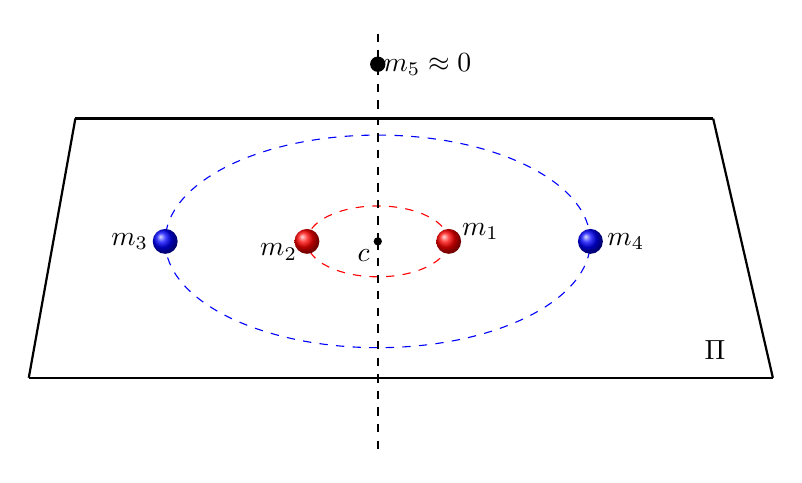
\begin{tikzpicture}[xscale=.9, yscale=.9]
				%Plano
				\draw[black,  line width=.8pt] (-6,0,-4.5)--(3,0,-4.5);
				\draw[black, line width=.8pt] (-3,0,5)--(7.5,0,5);
				\draw[black, line width=.8pt] (-3,0,5)--(-6,0,-4.5);
				\draw[black, line width=.8pt] (3,0,-4.5)--(7.5,0,5);
				%Elipses
				\draw[red,dashed] (0,0,0) ellipse (1cm and 0.5cm);
				\draw[blue,dashed] (0,0,0) ellipse (3cm and 1.5cm);
				%Cuerpos
					\shade[ball color=red]  (1,0) circle (5 pt);
					\node at (1.45,0.14) {$m_1$};
					\shade[ball color=red]  (-1,0) circle (5 pt);
					\node at (-1.4,-0.15) {$m_2$};

					\shade[ball color=blue]  (3,0) circle (5 pt);
					\node at (-3.5,0) {$m_3$};
					\shade[ball color=blue]  (-3,0)
					 circle (5 pt);
					\node at (3.5,0) {$m_4$};

					%eje z
        \draw[black, dashed, line width=.8pt] (0,0,0)--(0,3,0);
		\draw[black, dashed, line width=.8pt] (0,0,0)--(0,-3,0);
				% particula sin masa
		\draw[fill=black](0,2.5,0) circle (0.1 cm);
		\node at (0.7,2.5,0) {$m_5\approx 0$};
				%PI
				\node at (6.3,0,4) {$\Pi$};

				% CENTRO DE MASAS
				\draw[fill=black](0,0,0) circle (0.05 cm);
				\node at (-0.2,-0.2,0) {$c$};
\end{tikzpicture}\caption{Six-body problem}\label{fig:conf_esp}
\end{center}
\end{figure}


Problems like the one presented above have been extensively discussed in the literature. In \cite{sitnikov1960existence} K. Sitnikov considered the problem of two body in a Keplerian elliptic motion and a massless particle moving in the perpendicular line to the orbital plane passing
through the center of masses. Sitnikov obtained deep results about existence of solutions, for small $e>0$, with a chaotic behavior (see \cite[III(5)]{moser2016stable}). Periodic solutions for a Sitnikov configuration were considered in \cite{corbera2000periodic, corbera2002symmetric, llibre2008families,pustyl1990certain}.


Generalized circular Sitnikov problems, i.e. we have $n\geq 3$ primaries in a relative equilibrium motion,   were addressed more recently.
In \cite{soulis2008periodic} Soulis, Papadakis and Bountis studied existence, linear stability and bifurcations for a problem similar to $P$. They considered  a Lagrangian equilateral triangle configuration for the primary bodies, which were supposed to have the same mass $m_1=m_2=m_3$. In \cite{bountis2009stability} Papadakis and Bountis extended the results of \cite{soulis2008periodic} to $n$ primaries ($n\geq 3$) in a poligonal equal masses configuration. Later  in \cite{pandey2013periodic}, Pandey and Ahmad generalized  analysis started in \cite{soulis2008periodic} to the case with oblate primaries, i.e with space extended bodies.
In \cite{li2013characterization} Li, Zhang and Zhao studied a special type of
restricted circular $n+1$-body problem  with equal masses for the primaries in a regular polygon configuration. Periodic solutions for generalized Sitnikov problems with primaries performing  no rigid motions were studied in \cite{pustyl1990certain,rivera2013periodic}. In the previous papers the primary bodies are in the vertices of a regular polygon. In \cite{marchesin2013spatial} Marchesin and Vidal studied the problem $P$ for a rigid motion  of primaries in a  rhomboidal configuration.
 In \cite{bakker2015separating} Bakker and Simmons studied scape regions for the massless particle in a problem similar to $P$ for a certain type of periodic orbits for primaries including non homographic motions.


In the present paper, after introducing preliminaries facts in Section \ref{sec:pre},   we
obtain in Section \ref{sec:admisible.configuraciones} necessary and sufficient conditions on the configuration of primary bodies in order  that the $z$-axis to be invariant for the flow associated to the motion equations of the massless particle. For this type of configurations, that we call \emph{balanced}, the Sitnikov problem has sense.  In Section \ref{sec:addmisibles} we will find all balanced configurations for $n\leq 4$ primaries.  The Section \ref{sec:mas-mot} is devoted to describe all possible motion of the massless particle when the primaries are in a relative equilibrium (or rigid) motion. In this direction we observe that only are possible scape (both parabolic and hiperbolic) and periodic motions. Moreover, we will give a formula expressing the period of solutions  by means of integrals.  We prove in Corollary \ref{cor:sol.periodica.sist.completo} that the complete $n+1$-body system has  infinite quantity of periodic solutions. In Section  \ref{sec:sincro} we discuss the
situation when the entire system has a solution with the same period that the rigid motion of primaries. We call it synchronous solution. Surprisingly this fact is related to the existence of certain pyramidal central configurations (for the definition of this concept see \cite{fayccal1996classification,faycaltesis,ouyang2004pyramidal}). Finally, in the last section, we study certain non balanced configurations which allows some particular solutions of problem $P$.

In this paper we generalize and extend some results previously establish in the literature. For example our results in Section \ref{sec:mas-mot} generalize the results obtained by Marchesin and Vidal in \cite{marchesin2013spatial} for a rhomboidal configuration to any balanced configuration. In Section \ref{sec:sincro} we prove that there exists synchronous solutions for primaries in a regular poligonal equal mass configuration if and only if $2\leq n\leq 472$. The sufficient of this fact was established in \cite{li2013characterization}.


\section{Preliminaries}\label{sec:pre}

We start considering $n$  mass points, $n>2$, of masses $m_1,\ldots,m_n$ moving in a Euclidean 3-dimensional space according to Newton's laws of motion. We assume that $x_1(t),\ldots,x_n(t)$ are the coordinates (column vectors) of the bodies in some inertial Cartesian coordinate system. We denote by $r_{ij}=|x_i-x_j|$  the  Euclidean distance between $x_i$ and $x_j$. We can suppose, without any loos generality, that the center of mass   $c:=\sum_jm_jx_j/M$ ($M:=\sum_j m_j$) is fixed at the origin ($c=0$).

Initially we assume that the bodies are in a \emph{planar homographic motion} on the plane $\Pi$ (see \cite{JaumeLlibre276}). That means, assuming that  $\Pi$ is the plane determined by the first two coordinates axes, that

\begin{equation}\label{eq:x_j=rtQtq_j}
 x_j(t)=r(t)Q(\theta (t))q_j,
\end{equation}
where
\[
 Q(\theta )=\begin{pmatrix}
           \cos(\theta ) & -\sin(\theta ) & 0\\
           \sin(\theta ) & \cos(\theta ) & 0\\
           0            &     0     &  1\\
          \end{pmatrix}
\]
and $q_j\in\Pi$, $j=1,\ldots,n$ are vectors in a planar \emph{central configuration} (CC) in $\rr^3$, i.e. there exists $\lambda\in\rr$ such that
\begin{equation}\label{eq:def.CC}
\nabla_jU(q_1,\ldots,q_n)+\lambda m_jq_j=0,\quad j=1,\ldots,n.
\end{equation}
where the \emph{potential function} $U$ is defined by:
\begin{equation}\label{eq:potencial}
 U(x)=\sum_{i<j}\frac{m_im_j}{r_{ij}},
\end{equation}
and $\nabla_j$ denotes the $3$-dimensional partial gradient with respect to $x_j$. For simplicity we denote $q:=(q_1,\ldots,q_n)$.

According to \cite[Eq. (2.16)]{JaumeLlibre276}  the functions $r(t)$ and $\theta (t)$ solves the two-dimensional Kepler problems in polar coordinates, i.e.
\begin{equation}
 \begin{array}{rl}\label{eq:kepler.2.dim}
\ddot{r}(t)-r(t)\dot{\theta}(t)^2 & = -\frac{\lambda}{r(t)^2}\\
\frac{d }{dt}\left[ r(t)^2\dot{\theta}(t)\right] & =0.\\
\end{array}
\end{equation}
In the particular case of \emph{rigid motion}, we have  $r(t)\equiv 1$ and $\theta (t)=\sqrt{\lambda }t +\theta(0)$. Therefore the primaries bodies perform a periodic motion with period $T:=2\pi/\nu$, where $\nu^2=\lambda$.

Let $x_0(t)$ denotes the position of the massless particle.
According to the Newtonian equations of motion $q$ satisfies
\begin{equation}\label{eq:newton}
 \ddot{x}_0=\sum_{i=1}^n\frac{m_i(x_i-x_0)}{|x_i-x_0|^3}=:f(t,x_0).
\end{equation}





\section{Admissible configurations}\label{sec:admisible.configuraciones}
Henceforth we denote by $L$ the coordinate $z$ axis.
It is well know that a  necessary and sufficient condition for that $L$ be invariant under the  flow associated to the non autonomous system  \eqref{eq:newton}, is that $f(t,L)\subset L$ for all $t$, i.e. $L$ is \emph{$f$-invariant} for every $t$.


\begin{defi}
We say that a
central configuration $q$ is \emph{balanced} if and only if satisfies that for any $r>0$, such that the set
\[F_r:=\{i:|q_i|=r\}\]
is non empty, then
\begin{equation}\label{eq:suma0}\sum_{i\in F_r}m_iq_i=0.\end{equation}
i.e. every maximal set of  bodies which are equidistant from origin has center of mass equal to $0$.
\end{defi}



\begin{thm}\label{thm:prim} $L$ is $f$-invariant for every $t$ if and only  $q$ is balanced.
\end{thm}

For the proof of the previous theorem we need the following result


\begin{lem}\label{lem:1} For $c>0$ we define the function $y_c(t):=(c+t)^{-3/2}$. If $0<t_1<t_2<\ldots<t_k$ then the functions $y_j(t):=y_{t_j}(t)$  are linearly independent on  each open interval   $\mathcal{I}\subset \mathbb{R}^+$.
\end{lem}
\begin{proof} It is sufficient to prove that Wronskian

 \[W:=W(y_1,\ldots,y_k)(t)=\det\begin{pmatrix}
			      y_1 & \cdots & y_k\\
			      \frac{dy_1}{dt}&  \cdots & \frac{dy_k}{dt}\\
			      \vdots & \ddots & \vdots \\
			      \frac{d^{k-1}y_1}{dt^{k-1}}&  \cdots & \frac{d^{k-1}y_k}{dt^{k-1}}\\
                           \end{pmatrix}
\]
is not null on $\mathcal{I}$.

Using induction is easy to show that
\begin{equation}\label{eq:der_ind}\frac{d^iy_c}{dt^i}=\beta_{i}y_{c}^{\frac{2i+3}{3}},\quad\hbox{for some }\beta_{i}\neq 0, \hbox{ and for all }i=1,\ldots.
\end{equation}
Fix any $t\in I$. Then, according to \eqref{eq:der_ind} and writing $\lambda_j:=(t+t_j)^{-1}$, we have

\[
\begin{split}
  W(t)&=\det
    \begin{pmatrix}
      \lambda_1^{3/2} & \lambda_2^{3/2} &\cdots & \lambda_k^{3/2} \\
      \beta_1\lambda_1^{5/2} &\beta_1 \lambda_2^{5/2} &\cdots &\beta_1 \lambda_k^{5/2}\\
      \vdots & \vdots &\ddots & \vdots\\
      \beta_{k-1}\lambda_1^{k+1/2} & \beta_{k-1}\lambda_2^{k+1/2} &\cdots & \beta_{k-1}\lambda_k^{k+1/2}
    \end{pmatrix}
  \\
  &= \beta_1\beta_2\cdots\beta_{k-1} \lambda_1^{3/2}\lambda_2^{3/2}\cdots \lambda_k^{3/2}
     \det \begin{pmatrix}
      1& 1 &\cdots & 1 \\
      \lambda_1 & \lambda_2 &\cdots & \lambda_k\\
      \vdots & \vdots &\ddots & \vdots\\
      \lambda_1^{k-1} & \lambda_2^{k-1} &\cdots & \lambda_k^{k-1}
    \end{pmatrix}
  \\
  &= \beta_1\beta_2\cdots\beta_{k-1} \lambda_1^{3/2}\lambda_2^{3/2}\cdots \lambda_k^{3/2}
  \prod_{1\leq i<j\leq n}(\lambda_j-\lambda_i)
,
\end{split}
\]
where the last equality follows of the well known Vandermonde determinant identity. Therefore $W\neq 0$ if and only if $\lambda_i\neq\lambda_j$, $i\neq j$,
which in turn is equivalent to $t_i\neq t_j$, $i\neq j$.
\end{proof}








\begin{proof}[Proof of Theorem \ref{thm:prim}]
The condition $f(t,L)\subset L$ for all $t$ is equivalent to
\begin{equation}\label{eq:f(L)cL-->sum=0}
 \sum_{i=1}^n\frac{m_ir(t)Q(\theta (t))q_i}{\left(r(t)^2|q_i|^2+z^2\right)^{3/2}}=0,
\end{equation}
for every $t,z\in \rr$.

Let $D=\{|q_i|: i=1,\ldots,n\}$.  Suppose that $D=\{s_1,\ldots,s_k\}$, with $s_i\neq s_j$ for $i\neq j$, and  $\{1,\ldots,n\}=F_1\cup \cdots\cup F_k$, where if $i\in F_j$ then $|q_i|=s_i$. Then, multiplying equation \eqref{eq:f(L)cL-->sum=0} by $r(t)^2Q^{-1}(\theta(t))$  and writing $\zeta=(z/r(t))^2$ we have that \eqref{eq:f(L)cL-->sum=0} is equivalent to


\[\sum_{j=1}^k\left\{\frac{1}{(s_j^{2}+\zeta)^{3/2}}\sum_{i\in F_j}m_iq_i\right\}=0.\]
According to Lemma \ref{lem:1}, the last equation is equivalent to \eqref{eq:suma0}.
\end{proof}


\section{Admissible collisionless configurations for $n\leq 4$}\label{sec:addmisibles}

In this section we find all balanced collisionless configuration with $n\leq 4$. We observe that the collisionless condition for a configuration $q_1.\ldots,q_n$ implies that $q_i\neq 0$ for $i=1,\ldots,n$. From the fact that the center of masses is an excluded position we obtain
\begin{equation}\label{F_r.no.vac-->CF_r.geq2}
 F_r\neq \emptyset \Rightarrow \# F_r\geq 2.
\end{equation}



Trivially, a configuration of two point masses $m_1$ and $m_2$ is balanced if and only if $m_1=m_2$.

If $n=3$, from \eqref{F_r.no.vac-->CF_r.geq2}, the configuration consists of three equidistant bodies from the origin. Therefore, it must to be the Lagrangian equilateral triangle configuration. Now, by equation \eqref{eq:suma0} and an elementary geometrical reazoning   we have that $m_1=m_2=m_3$.

The case $n=4$ is more interesting. We will use the following result which can be seen in \cite{moeckel1990central}.

``Let $q$ be a planar configuration. For each pair, $i$, $j$, the line
containing $q_i$ and $q_j$ together with its perpendicular bisector form axes which
divide the plane into four quadrants. The union of the first and third quadrants
is an hourglass shaped region which will be called a `cone'; similarly,
the second and fourth quadrants together form another cone. The phrase `open
cone' refers to a cone minus the axes.''

\begin{thm}[Perpendicular Bisector Theorem]\label{thm:bisector.moeckel}
Let $q$ be a planar central configuration and let
$q_i$ and $q_j$ be any two of its points. Then if one of the two open cones determined
by the line through $q_i$ and $q_j$ and its perpendicular bisector contains points of
the configuration, so does the other one.
\end{thm}

Next we characterize all the $4$-body admisible collisionless configurations.

\begin{thm}\label{thm:caracterizacion4}
Let $q$ be a 4-body central configuration. Then $q$ is  admisible and collisionless if and only if,  for a suitable enumeration  of bodies,   $q_1=-q_3$, $q_2=-q_4$, $m_1=m_3$,  $m_2=m_4$, and  $q$ is of some of the following mutually exclusive types:
\begin{description}
\item[CCcl.]   collinear,
\item[CCr.]  a rhombus with $r_{13}<r_{24}$ and $m_1>m_2$,
\item[CCs.]  a square with four equal masses.
\end{description}
\end{thm}







\begin{proof}
Since \eqref{F_r.no.vac-->CF_r.geq2} we have two cases.

\emph{Case 1.}  $m_1\geq m_2$, $|q_1|\neq|q_2|$, $|q_1|=|q_3|$ and $|q_2|=|q_4|$. Now \eqref{eq:suma0} implies that
 $m_1=m_3$, $m_2=m_4$, $q_1=-q_3$ and $q_2=-q_4$.  We divide the plane in two cones $C_i$, $i=1,2$, by means of  the line $P$ joining $q_1$  and $q_3$ together with its perpendicular bisector $M$.  From Theorem \ref{thm:bisector.moeckel}, if  $q_2$  is in $C_1$, then  $q_4$ is in $C_2$, and vice versa. This is a contradiction with the fact that $q_2=-q_4$. Then $q_2,q_4\in P$ or $q_2,q_4\in M$, i.e. $q$ is collinear or is a rhombus with equal masses in opposite vertices. In the first case, $q$ is of  CCcl type. In the second case, if $m_1>m_2$,   was proved in \cite[Eqs. $(3.44)$ and $(3.45)$]{long2002four} that $r_{13}<r_{24}$, hence $q$ is of  CCr type. From \cite[Corollary 2]{perez2007convex} if $m_1=m_2$ then the configuration is a square witch is a contradiction with the fact that $|q_1|\neq|q_2|$.

\emph{Case 2.} $|q_1|=|q_2|=|q_3|=|q_4|$. In this situation,  was proved in \cite{hampton2005co} that the configuration is the equal mass square.
\end{proof}

\section{Massless particle motion}\label{sec:mas-mot}
In this section we analyze all possible motions for the massless particle $x_0$. In particular we will see that all motion is periodic or is a scape trayectory. We will find that there exists $T_0$-periodic solutions for all $T_0$ in an interval  $(\sigma(q),+\infty)$. This fact implies that there exists an infinity quantity of periodic solutions for the entire $n+1$-body system.



In this and next sections we suppose that the primaries bodies are in a $T$-periodic rigid motion asociate to an admisible collisionless $q$, i.e  $r(t)\equiv 1$ and from the remark follows \eqref{eq:kepler.2.dim}, $\theta (t)=\sqrt{\lambda}t$. Without loss of generality,  we have assumed that $\theta(0)=0$. For the particle, we assume that it is moving on $L$. Therefore, we assume that $x_0(t)=(0,0,z(t))$. According to Theorem \ref{thm:prim}, $x_0$ is solution of \eqref{eq:newton}, if and only if $z(t)$ is solution of the autonomous equation


\begin{equation}\label{eq:eq_new_red}
 \ddot{z}=-\sum_{i=1}^n\frac{m_iz}{(s_i^2+z^2)^{3/2}},
\end{equation}
where $s_i=|q_i|$.

The second order equation \eqref{eq:eq_new_red} is consevative, therefore solutions conserve the energy
\begin{equation}\label{eq:conser.energ}
E(z,v):=\frac{|v|^2}{2}-\sum_{i=1}^{n} \frac{m_i}{\left(s_i^2+z^2\right)^{\frac12}},
\end{equation}
i.e. $E(z(t),\dot{z}(t))$ is constant.



Following \cite{marchesin2013spatial} we introduce the next concepts.
\begin{defi}
 A solution $z(t)$ of \eqref{eq:eq_new_red} such that  $\lim\limits_{t\to\infty}z(t)=\infty$ is called hyperbolic for $t\to \infty$ when $\lim\limits_{t\to\infty}\dot{z}(t)= z_{\infty}\neq 0$ and is called parabolic if $\lim\limits_{t\to\infty}\dot{z}(t)=0$.
\end{defi}






The following theorem characterize all the possible motions for the massless particle.

\begin{thm}\label{thm:prin_ine} We assume that $q$ is a admisible collisionless configuration and the primaries are in a rigid motion. Every solution of \eqref{eq:eq_new_red} if of the some following types:
\begin{enumerate}
\item\label{1} Hyperbolic, when $E>0$,
\item\label{2} Parabolic, when $E=0$,
\item\label{3} Periodic, when $E_{min}:=-\sum_{i=1}^{n}\frac{m_i}{s_i}<E<0$.
\item\label{4} Equilibrium solution when $E=E_{min}$.
\end{enumerate}
\end{thm}

\begin{proof}
We follow a standard argument for hamiltonian systems (see \cite{rivera2012bifurcacion}).

We plot the level sets of $S(E)=\{(z,v):E(z,v)=E\}$, in the phase space $(z,v)$,  for different values of $E$. An elementary analysis shows that
\begin{itemize}
 \item If $E\geq 0$ then $S(E)$ is the union of two bounded graphs. They are symmetric with respect to $z$-axis, each of which is contained  in some semiplane $v> 0$ or $v<0$. The $v$-positive branch is the graph of a function $v(E,z)$, which  is decreasing with respect to $|z|$. Moreover, $\lim\limits_{|z|\to \infty}v(E,z)=\sqrt{2E}$.

 \item For every $E\geq E_{min}$, the energy curve cut the $v$-axis at $\pm(2E+2\sum_{i=1}^n m_is_i^{-1})^{\frac12}$.

 \item If $E_{min}<E<0$ then $S(E)$ is a simple closed curve symmetric with respecto to $z$ and $v$ axes.

 \item  An energy curve cut the $z$-axis, only in the case that $E<0$, at $\pm z_{E}$, where $z_E$ is the only positive solution of $-\sum_{i=1}^n m_i (s_i^2+z_{E}^2)^{-\frac12}=E$.
\end{itemize}

In the figure  \ref{fig:conf_esp} we show the phase portrait for two equal masses primaries.

The function $\varphi(t)=(z(t),\dot{z}(t))$ solves the system $\dot{\varphi}(t)=F(\varphi(t))$, where $F(z,v)=(v,-\sum_{i=1}^{n}m_iz (s_i^2+z^2)^{-3/2})$. The only stationary point of $F$ is $(z,v)=(0,0)$. Therefore, the level surfaces $S(E)$, with $E\neq E_{min}$, not contains stationary points. A well know argument implies that the trayectories $t\mapsto (z(t),\dot{z}(t))$  fill completely the energy curves.

We note that if $E\geq 0$ and $v(E,0)>0$ ($v(E,0)<0$) then $z(t)$ is increasing (decreasing) with respect to $t$. For all the above if $E\geq 0$ then $|z(t)|\to \infty$ when $t\to \infty$. Moreover $\lim\limits_{t\to\infty}\dot{z}(t)=\pm\sqrt{2E}$.  From this we conclude that the trayectory is hyperbolic when $E>0$ and it is parabolic in the case $E=0$.

In the case that $E_{min}<E<0$ we have that the trayectory is contained in a closed curve, therefore it is periodic orbit.

Finally if $E=E_{min}$ clearly we have that $z(t)\equiv 0$.
\begin{figure}[h]
\begin{center}
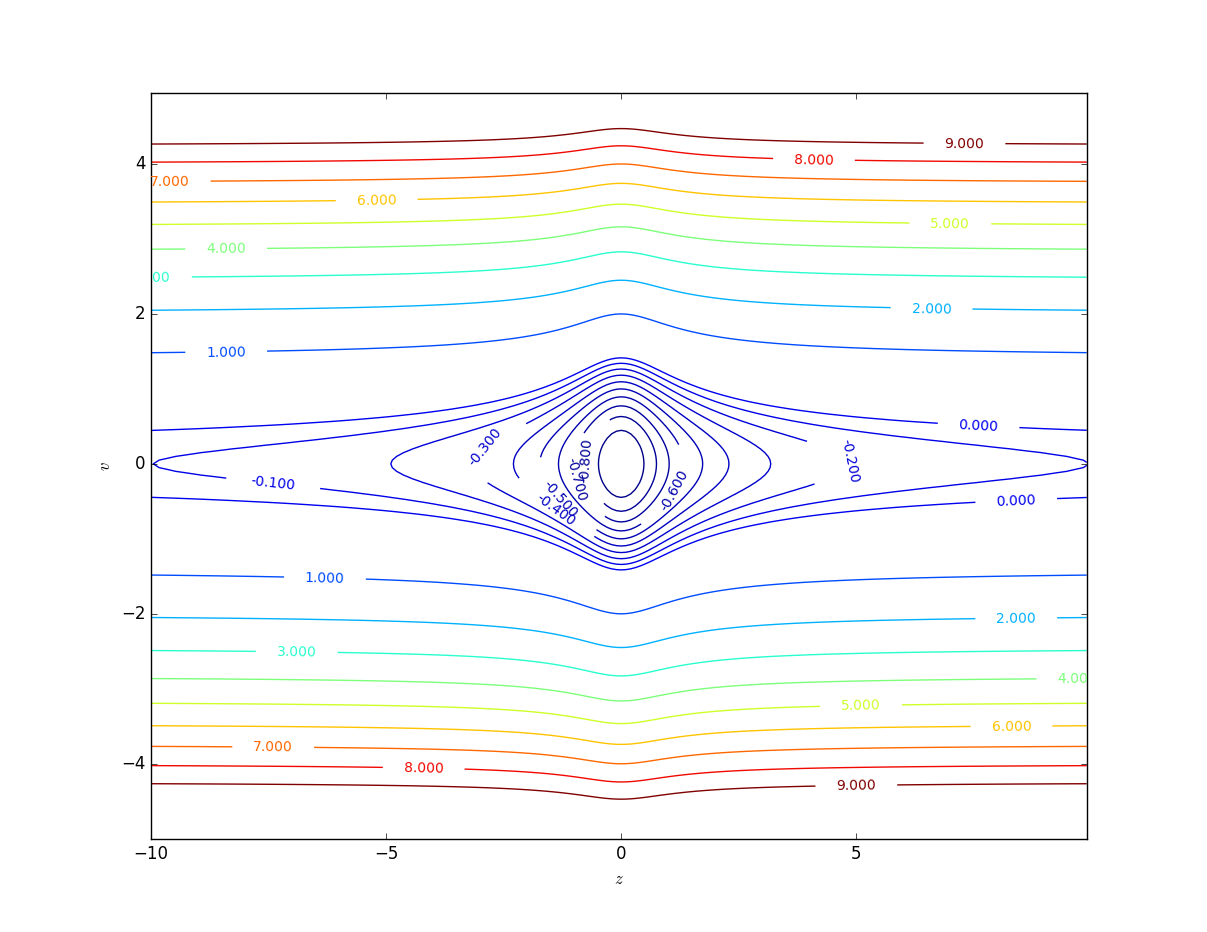
\includegraphics[scale=0.3]{figure_1.png}
\caption{Energy level for two equal mass primaries}\label{fig:energy}
\end{center}
\end{figure}
\end{proof}

\begin{thm}\label{thm:prop.periodos}
We denote by $T_0(E)$ the minimal period for a solution of \eqref{eq:eq_new_red} with $E_{min}<E<0$. Then
\begin{enumerate}
 \item\label{it:T0.formula} for $z_E$ the only positive solution of $-\sum_{i=1}^n m_i (s_i^2+z_{E}^2)^{-\frac12}=E$
 \begin{equation}\label{eq:form.T0E-periodo}
 T_0(E)=2^{3/2}\int_{0}^{z_E} \left(E+\sum_{i=1}^n m_i (s_i^2+z^2)^{-\frac12}\right)^{-\frac12} dz,
 \end{equation}
 \item\label{it:T0.creciente} $T_0(E)$ is an increasing function.
 \item\label{it:T0.rango} $T_0\left((E_{min},0)\right)=(T_{min},+\infty)$, where  $T_{min}=2\pi\left(\sum_{i=1}^n\frac{m_i}{s_i^3} \right)^{-1/2}$.

 \end{enumerate}
\end{thm}

\begin{proof}
Let $E_{min}<E<0$ and let $z(t)$ be a solution with $z(0)=0$ and $\dot{z}(0)=\sqrt{2(E-E_{min})}$. Then $E(z(0),\dot{z}(0))=E$. Therefore $z(t)$ is $T_0(E)$-periodic. As a consequence of the symmetries of the equation we have that $z(T_0(E)/4)=z_E$. Then, taking account \eqref{eq:conser.energ} we have that
\begin{equation*}
 \begin{split}
  \frac{T_0}{4}&=\int_0^{T_0/4}\left(E+\sum_{i=1}^n m_i (s_i^2+z^2)^{-\frac12}\right)^{-\frac12} z'(t) dt\\
  &=\frac{1}{\sqrt{2}}\int_{0}^{z_E} \left(E+\sum_{i=1}^n m_i (s_i^2+z^2)^{-\frac12}\right)^{-\frac12} dz,
 \end{split}
\end{equation*}
and we have proved item \textit{1}. In order to prove item \textit{2} we note that
\begin{equation*}
 \begin{split}
  2^{-3/2}T_0(E)
  &=
    \int_0^{z_E}\left(\sum_{i=1}^n m_i \left((s_i^2+z^2)^{-\frac12}-(s_i^2+z_E^2)^{-\frac12}\right)\right)^{-\frac12}dz\\
  &=\int_0^{z_E} \left(z_E^2-z^2\right)^{-\frac12} f(z,z_E)dz\\
  &=\int_0^1 \left(1-u^2\right)^{-\frac12} f(z_Eu,z_E)du,
 \end{split}
 \end{equation*}
where \[f(z,z_E)=\left(\sum_{i=1}^n m_i \left\{(s_i^2+z^2)(s_i^2+z_E^2)\right\}^{-\frac12} \left\{(s_i^2+z^2)^{\frac12}+(s_i^2+z_E^2)^{\frac12} \right\}^{-1}\right)^{-\frac12}.\]
We note that $f(z_Eu,z_E)$ is a increasing function with respect to $z_E$ for $u\in [0,1]$ fix. This implies item \ref{it:T0.creciente}.

On the other hand
\begin{equation*}
 \lim\limits_{z_E \to 0}f(z_Eu,z_E)=\left(\sum_{i=1}^{n} \frac{m_i}{2s_i^3}\right)^{-\frac12} \quad \text{and}\quad  \lim\limits_{z_E \to \infty}f(z_Eu,z_E)=\infty.
\end{equation*}
Therefore, from the dominated convergence theorem and monotone convergence theorem we have that
\[\lim\limits_{z_E\to 0}T_0=2\pi\left(\sum_{i=1}^{n} \frac{m_i}{s_i^3}\right)^{-\frac12}\quad \text{and}\quad \lim\limits_{z_E\to \infty}T_0=\infty.\]
Finally,  since $T_0=T_0(z_E)$ is continuous and increasing respect to $z_E$ we conclude the afirmation in the item \ref{it:T0.rango}.
\end{proof}

\begin{comentario}
 It si posible to use the classical theory of hamiltonian systems (see \cite{A}) to derive the formula \eqref{eq:form.T0E-periodo} (see \cite{acinas2014estimates} for a related problem).
\end{comentario}



\begin{comentario}
Let us to show a second proof of item \ref{it:T0.rango} of Theorem \ref{thm:prop.periodos}.

The inequality $T_0>T_{min}$ is consequence of comparison Sturm's theorem applied to equations  $z''+q_1(z)z=0$, where $q_1(z)=\sum_{i=1}^{n} m_i \left(s_i^2 +z^2\right)^{-3/2}$, and $z''+\left(\sum_{i=1}^{n} m_i s_i^{-3}\right)z=0$. This prove that $T_0\left((E_{min},0)\right)\subset(T_{min},+\infty)$.

For the reverse inclusion  we  follow arguments of \cite{zhao2015nonplanar} and \cite{li2013characterization}, based on variational principles.


Let $T_0>T_{min}$. We consider the action integral
\[\mathcal{I}(z)=\int_0^{T_0}\frac12|z'|^2+\sum_{i=1}^n\frac{m_i}{\sqrt{s_i^2+z^2}}dt,\]
Then $T_0$-periodic solutions of \eqref{eq:eq_new_red} are critical points of $\mathcal{I}$ in the space $H^1(\mathbb{T},\rr)$, where $\mathbb{T}=\rr/T_0\mathbb{Z}$, of the functions  absolutely continuous, $T_0$-periodic with $z'\in L^2(\mathbb{T},\rr)$ (see \cite[Cor. 1.1]{Mawhin2010}). We prove the existence of critical points by means of the direct method of calculus of variations, i.e. we will prove that $\mathcal{I}$ has minimum.  The functional $\mathcal{I}$ is not coercive in $H^1(\mathbb{T},\rr)$,  this deficiency is drawn with symmetry techniques (see \cite{David-2004}). The group $\mathbb{Z}_2$ acts on $H^1(\mathbb{T},\rr)$ according to the following assignments $(\bar{0}\cdot z)(t)=z(t)$ and $(\bar{1}\cdot z)(t)=-z(t+\frac{T_0}{2})$. The functional $\mathcal{I}$ is $\mathbb{Z}_2$-invariant, i.e. $\mathcal{I}(g\cdot z)=\mathcal{I}(z)$. We define the space of all $\mathbb{Z}_2$-symmetric (this simmetry is called the italian simmetry) funcions \[\Lambda(\mathbb{T},\mathbb{R}):
=\left\{ z\in H^1(\mathbb{T},\rr) | \forall g\in \mathbb{Z}_2 : z=g\cdot z \right\}.\]
The funciontal $\mathcal{I}$ restricted to $\Lambda$  is coercive. This fact follows from an obvious adaptation of proposition 4.1 of \cite{David-2004}. We note that $F(z):=\sum_{i=1}^nm_i(s_i^2+z^2)^{-\frac{1}{2}}$ satisfies the condition $(A)$ in \cite[p. 12]{Mawhin2010}, then $\mathcal{I}$  is continuously differentiable and weakly lower semicontinuous on $H^1(\mathbb{T},\rr)$ (see \cite[p. 13]{Mawhin2010}). Therefore $\mathcal{I}$ has a minimum $z_0$ in $\Lambda(\mathbb{T},\mathbb{R})$. Then by the Palais' principle symmetric criticality,  $z_0$ is a critical point of $\mathcal{I}$ in $H^1(\mathbb{T},\rr)$ (see \cite{David-2004} and \cite{RichardPalais274}).

We use the second variation $\delta^2 \mathcal{I}$ in order to show  that $z_0\nequiv 0$. It is well known (see \cite[Th. 1.3.1]{jost1998calculus}) that if $z_0$ is a minimum of $\mathcal{I}$ on $H^1(\mathbb{T},\rr)$  then $\delta^2 \mathcal{I} (z_0,\varphi)\geq 0$ for all $\varphi\in H^1(\mathbb{T},\rr)$. In our case
\[\delta^2\mathcal{I}(0,\varphi)=\int_0^{T_0} |\varphi'|^2-\sum_{i=1}^{n}\frac{m_i}{s_i^3}\varphi^2 dt,\]
(see \cite[Eq. 1.3.6]{jost1998calculus}). In particular for $\varphi(t)=\sin (2\pi t/T_0)$ it follows from $T_0>T_{min}$  that
\begin{equation}\label{eq:form.delta2}
 \delta^2 \mathcal{I} (0,\varphi)=\left( \frac{4\pi^2}{T_0^2}-\sum_{i=1}^{n}\frac{m_i}{s_i^3} \right)\frac{T_0}{2}<0.
\end{equation}
It is sufficient  to guarantee that $z_0\equiv 0$ is not a minimum.


This second proof, unlike the first one, does not guarantee that $T_0$ is the minimum period for $z_0$. It could happen that $z_0$ had period $T_0/m$, with natural $m\in\mathbb{N}$. Because of Italian symmetry this $m$ should be odd.
\end{comentario}






\begin{cor}\label{cor:sol.periodica.sist.completo}
The complete $n+1$-body has a infinity quantity of periodic solutions.
\end{cor}
\begin{proof}
Let $l/m$  be a rational number with $Tl/m>T_{min}$. Then, there exists a solution of the entire system with period $lT$.
\end{proof}





\section{Synchronous solutions and pyramidal CC}\label{sec:sincro}



If the equation \eqref{eq:eq_new_red} has a $T$-periodic solution,  we say that the solution is \emph{synchronous}. In \cite{li2013characterization} was studied the existence of synchronous solutions for $n$ equal mass primary bodies in a regular polygon configuration.

In this section we establish a relation between the existence of synchronous solutions and the concept of pyramidal central configuration (see \cite{fayccal1996classification,faycaltesis,ouyang2004pyramidal}).

\begin{defi}
A central configuration of $n+1$ mass point $q_1,\ldots,q_{n+1}$ in $\rr^{3}$  is called a pyramidal central configuration (PCC) if and only if $n$ points, we say $q_1,\ldots,q_n$, are in some plane $\Pi$ and $q_{n+1}$ is not.
\end{defi}

The following lemma was proved in \cite{ouyang2004pyramidal} (see also \cite{faycaltesis})
\begin{lem}[\cite{ouyang2004pyramidal}, Lemma 2.1]\label{lem:PCC}
 Let $q_0,\ldots,q_{n}$ be a PCC such that $m_{0}$ is off the plane containing $m_1,\ldots,m_n$. If $m_{0}>0$ then $m_{0}$ is equidistant from $m_1,\ldots,m_n$.
\end{lem}

We remark that the condition $m_{0}>0$ is important in the previous Lemma. We will show below examples of two PCC with $m_{0}=0$ which do not satisfy the conclusion of  Lemma \ref{lem:PCC}.



\begin{prop}\label{cor:sol.sincronica}
We assume that $q=q_1,\ldots,q_n$ is an admisible collisionless configuration and that the primaries are in a rigid motion. Then, there is a synchronous solution if and only if there exists $c\in \rr$ such that the points $q_0,\ldots,q_{n}$ associated to the masses $m_0,\ldots,m_{n}$, with $q_{0}=(0,0,c)$ and $m_{0}=0$, form a PCC.
\end{prop}

\begin{proof}
We start assuming that there exist a synchronous solution. As a consequence of the Theorem \ref{thm:prop.periodos}(\ref{it:T0.rango}) and the fact that $T^2=4\pi^2/\lambda$ we have that

 \begin{equation}\label{eq:lamdbda<suma.si3}
\lambda<\sum_{i=1}^n\frac{m_i}{s_i^3}.
 \end{equation}
 Since $\sum_{i=1}^{n}m_i\left(s_i^2+c^2\right)^{-3/2}\to 0$, when $c\to +\infty$, there exists $c\in \rr$ such that
 $ \sum_{i=1}^{n}m_i\left(s_i^2+c^2\right)^{-3/2}=\lambda$. Therefore
 \begin{equation}\label{eq:cond.CC1}
  -\sum_{i=1}^{n}\frac{m_i c}{\left(s_i^2+c^2\right)^{3/2}}=-\lambda c.
 \end{equation}
As $q_1,\ldots,q_n$ is an admisible configuration then
\begin{equation}\label{eq:cond.CC2}
   \sum_{i=1}^{n}\frac{m_i q_i}{\left(s_i^2+c^2\right)^{3/2}}= (0,0).
\end{equation}
We define  $q_{n+1}:=(0,0,c)$ and $m_{n+1}=0$. The equations \eqref{eq:cond.CC1}, \eqref{eq:cond.CC2}  and the facts that $q_1,\ldots,q_n$ is a CC, with constant $\lambda$,  implies that $q_1,\ldots,q_{n+1}$ and $m_1,\ldots,m_{n+1}$  form a PCC.

The proof of the reciprocal statement follows in a direct way.
\end{proof}

\begin{cor}
We assume that $q=q_1,\ldots,q_n$ is an admisible collisionless configuration and that the primaries are in a rigid motion. Then, there is a synchronous solution if and only if
 \begin{equation}\label{eq:ine_prin}
 \sum_{i<j}\frac{m_im_j}{r_{ij}}<\left(\sum_{i=1}^n\frac{m_i}{s_i^3}\right)\left(\sum_{i=1}^nm_is_i^2\right).
\end{equation}
\end{cor}

\begin{proof}
The result is consequence of \eqref{eq:lamdbda<suma.si3} and the fact that $T^2=4\pi^2 \sum_{i=1}^{n}m_i|q_i|^2/U$   (see \cite[p. 109]{JaumeLlibre276}).
\end{proof}







The sufficiency of the condition $n\leq 472$ in the following corollary  was proved in \cite{li2013characterization}.

\begin{cor}\label{cor:nleq472}
We suppose that $q$ is the equal masses regular polygon configuration  (this is an admisible CC). Then there exists a synchronous solution if and only if $2\leq n\leq 472$.
\end{cor}

\begin{proof}
In this case $s_1=s_2=\cdots=s_n=:r$ and $m_1=m_2=\cdots=m_n=:m$. Then, from the law of cosines we obtain
\[
 \sum_{i<j}\frac{m_im_j}{r_{ij}}=\frac{nm^2}{4r}\sum_{j=1}^{n-1}\frac{1}{\sin\left(\frac{j\pi}{n}\right)}.
\]
Therefore the condition \eqref{eq:ine_prin} is equivalent to

\begin{equation}\label{eq:ine_prin_LShShao}
  \frac1n\sum_{j=1}^{n-1}\frac{1}{\sin\left(\frac{j\pi}{n}\right)}<4.
\end{equation}

This inequality was also derived by Li, J. et al. in \cite{li2013characterization}, where the authors proved (performing computer calculations) that inequality \eqref{eq:ine_prin_LShShao} holds true for $2\leq n\leq 472$. Let us prove that any other $n$ does not satisfies \eqref{eq:ine_prin_LShShao}.


Using that $1/\sin (x)$ is a convex function on $[0,\pi]$ and the composite trapezoid rule (see \cite{kincaid1991numerical}) we have that
\[
\begin{split}
 \int_{\frac{\pi}{n}}^{\frac{n-1}{n}\pi}\frac{1}{\sin (x)}dx&\leq \frac{\pi}{2n}\left\{ \frac{1}{\sin(\frac{\pi}{n})} + \frac{1}{\sin(\frac{n-1}{n}\pi)} +2\sum_{j=2}^{n-2}\frac{1}{\sin(j\frac{\pi}{n})} \right\}\\
 &=\frac{\pi}{n}\sum_{j=1}^{n-2}\frac{1}{\sin(j\frac{\pi}{n})}.
\end{split}
\]
Therefore
\[
\begin{split}
 \frac1n \sum_{j=1}^{n-1}\frac{1}{\sin\left(\frac{j\pi}{n}\right)}&\geq \frac{1}{\pi}\int_{\frac{\pi}{n}}^{\frac{\pi(n-1)}{n}}\frac{1}{\sin (x)}dx+\frac{1}{n\sin\left(\frac{n-1}{n}\pi\right)}\\
 &=\left.\frac{1}{2\pi}\log \left( \frac{1-\cos(x)}{1+\cos(x)}\right)\right|_{\frac{\pi}{n}}^{\frac{n-1}{n}\pi}+\frac{1}{n\sin\left(\frac{\pi}{n}\right)}\\
 &=\frac{1}{\pi}\left\{\log \left(\frac{1+\cos(\frac{\pi}{n})}{1-\cos(\frac{\pi}{n})}\right)+\frac{\pi/n}{\sin\left(\frac{\pi}{n}\right)}\right\}\\
 &=:f\left(\frac{\pi}{n} \right).
 \end{split}
\]
It is easy to see that $f(x)$ is a decreasing function on $(0,\pi/2)$. Moreover $f(\pi/842)\approx 4.0006>4$. Therefore, if $n\geq 842$ then $n$ does not satisfies inequality \eqref{eq:ine_prin_LShShao}. The validity of the inequality \eqref{eq:ine_prin_LShShao}, for $n\leq 841$, is easily checked using computer. This gives the result that the inequality holds for all $n \leq 472$.
\end{proof}




Our next objective is to verify that condition \eqref{eq:ine_prin} is satisfied for all balanced CC of 3-body or 4-body. Since we have already proved, in  Corollary \ref{cor:nleq472}, that \eqref{eq:ine_prin} holds for a equilateral triangle and square configurations of equal masses bodies, it only rest to prove, in virtue of Theorem \ref{thm:caracterizacion4}, the following result.



\begin{thm}\label{thm:CC.3.4.satis.cond.adm}
The central configurations CCcl and CCr satisfy condition \eqref{eq:ine_prin}.
\end{thm}



\begin{proof}

Let's start by analyzing the central configuration CCr. We can suppose without loss of generality that $ q_1 = -q_3 = (0, y) $ for $ y> 0 $, $ q_2 = -q_4 = (1,0) $. Recall that $ y <1 $. The condition \eqref{eq:ine_prin} becomes
\[\frac{m_1^2}{2y}+\frac{4m_1m_2}{\sqrt{1+y^2}}+\frac{m_2^2}{2}<\left(\frac{2m_1}{y^3}+2m_2\right) \left(2m_1y^2+2m_2\right).\]
As $m_1^2/(2y)<4m_1^2/y$, $m_2^2/2<4m_2^2$ and $4m_1m_2/\sqrt{1+y^2}<4m_1m_2/y^3$ (since $y<1$), we have that the inequality holds.

 Now we consider the central configuration CCl.  We can suppose without loss of generality that $q_1=-q_3=1$, $q_2=-q_4=x$ with $0<x<1$, and $m_1=m_3=\mu$, $m_2=m_4=1-\mu$, with $0<\mu<1$.  Then the inequality \eqref{eq:ine_prin} becomes
\[\frac{2\mu(1-\mu)}{1-x} +\frac{2\mu(1-\mu)}{1+x}+\frac{\mu^2}{2}+\frac{(1-\mu)^2}{2x}<4\mu^2+4\mu(1-\mu)x^2+\frac{4\mu(1-\mu)}{x^3}+\frac{4(1-\mu)^2}{x}.\]
As $ \mu ^ 2/2 <4 \mu^2$ and $ (1-\mu)^2/(2x)< 4(1-\mu)^2/x $ (without taking into account the term $4\mu(1- \mu)x^2$) we just have to show that
\[\frac{2\mu(1-\mu)}{1-x} +\frac{2\mu(1-\mu)}{1+x}<\frac{4\mu(1-\mu)}{x^3},\]
and this is equivalent to see that
\begin{equation}\label{eq:ineq.4.cuerpos.alinea}
\frac{x^3}{1-x^2}<1.
\end{equation}
The values of $x$ involved in the above inequality are such that the configuration for the vector mass $(\mu,1-\mu,1-\mu,\mu)$ is central, by Moulton \cite{moulton1910straight}, fixed a mass $\mu$ there is only one value $x$ satisfiying this condition. So, we can define $x(\mu)$ as such value of $x$.  We note that $x^3/(1-x^2)$ is an increasing function with respect to $x\in (0,1)$ and it is less than $1$ for $x\in (0,3/4)$. Hence, if we could prove that $x(\mu)$ is a decreasing function and
\begin{equation}\label{eq:ineq.4.cuerpos.lim0}
\lim\limits_{\mu\to 0}x(\mu)<3/4
\end{equation}
we would have justified \eqref {eq:ineq.4.cuerpos.alinea}.

Let's first prove that $x(\mu)$ is a decreasing function. Replacing $q_j^0$, $m_j$ and eliminating $\lambda$ from the equations \eqref{eq:def.CC} we get
\[\frac{\mu}{4} - \frac{\mu}{x \left(x + 1\right)^{2}} + \frac{\mu}{x \left(- x + 1\right)^{2}} + \frac{- \mu + 1}{\left(x + 1\right)^{2}} + \frac{- \mu + 1}{\left(- x + 1\right)^{2}} - \frac{1}{x^{3}} \left(- \frac{\mu}{4} + \frac{1}{4}\right) = 0\]
which is equivalent to
 \[\mu=- \frac{8 x^{5} - x^{4} + 8 x^{3} + 2 x^{2} - 1}{\left(x - 1\right) \left(x + 1\right) \left(x^{5} - 9 x^{3} + x^{2} - 1\right)}.\]
Therefore
\[
 \frac{d\mu}{dx}=\frac{x^{2} \left(16 x^{9} - 3 x^{8} + 32 x^{7} + 12 x^{6} - 304 x^{5} - 2 x^{4} + 44 x^{2} - 51\right)}{\left(x - 1\right)^{2} \left(x + 1\right)^{2} \left(x^{5} - 9 x^{3} + x^{2} - 1\right)^{2}}.
\]
Clearly $d\mu/dx<0$ for $x\in (0,1)$. Which, in turn, implies that $x$ is decreasing respect to $\mu$.





Let's see now that \eqref{eq:ineq.4.cuerpos.lim0} holds. When $\mu$ goes to $0$, $x(\mu)$ converges to the only solution, $x(0)$, in the interval $(0,1)$ of the equation $8 x(0)^{5} - x(0)^{4} + 8 x(0)^{3} + 2 x(0)^{2} - 1=0$.  Then  $ 8 x(0)^{3} -1< 0$ which implies that $x(0)<3/4$ as we wanted to prove.
\end{proof}


\begin{comentario}
As consequence of previous results there exist five-body $PCC's$ with $m_1,\ldots,m_4$  in a CCcl or CCr configuration and $m_0=0$ is in the  line perpendicular to plane containing $m_1,\ldots,m_4$ passing by the mass center. These are examples of $PCC's$ wich does not verify the conclusion of Lemma \ref{lem:PCC}.

 The configuratios CCcl and CCr are bases of a PCC, with a vertix out of the plane , which do not verify the conclusion of Lemma \ref{lem:PCC}.
\end{comentario}


\begin{cor}
For all  balanced CC of 3-body or 4-body  problem $P$ has a synchronous solution.
\end{cor}
























\section{Non balanced central configurations}

The following result shows a necessary condition for that  a non-balanced CC allows a solution of the problem $P$.

\begin{thm}\label{thm:no.admisible.movimiento}
We suppose that $q$ is a non admisible CC and  that the primaries are in a homographic motion, i.e.  equation \eqref{eq:x_j=rtQtq_j} is satisfied. Assume that the massless particle is moving on the $z$-axis with position vector $x_0(t)=(0,0,z(t))$. Then, some of the following statement is satisfies:
\begin{enumerate}
 \item\label{it:z==0} The massless particle is in a stationary motion and
 \begin{equation}\label{eq:acel.centrmasa=0}
  \sum_{i=1}^{n}\frac{m_iq_i}{s_i^3}=0,
 \end{equation}
 i.e. the positions $0,q_1,\ldots,q_n$ and the masses $0,m_1,\ldots,m_n$ are in a CC.
 \item\label{it:z=r} The $n+1$-body system is in a homothetic motion. i.e. $Q(\theta(t))$ in the equation \eqref{eq:x_j=rtQtq_j} is the identity matrix and $z(t)=cr(t)$, for some constant $c$. Moreover, the configuration $q_0,\ldots,q_n$ is a PCC, where $q_0=(0,0,c)$ and $m_0=0$.
\end{enumerate}
\end{thm}

\begin{proof}
 We recall the definition of the function $f$ and line $L$ from the Section \ref{sec:admisible.configuraciones}.

The fact of the massless particle is moving on $L$, is equivalent to the condition $f(t,x_0(t))\in L$ for all $t$, which, instead, is equivalent to the equality
\begin{equation}\label{eq:z/r}
 \sum_{i=1}^n\frac{m_ir(t)Q(\theta (t))q_i}{\left(r(t)^2|q_i|^2+z(t)^2\right)^{3/2}}=0,
\end{equation}
for every $t\in \rr$.

With the same notation and following similar reasoning that in the proof of Theorem \ref{thm:prim}, we prove that
\begin{equation}\label{eq:sumr.sumFr_miqi=0}
\sum_{j=1}^k\left\{\frac{1}{(s_j^{2}+(z(t)/r(t))^2)^{3/2}}\sum_{i\in F_j}m_iq_i\right\}=0.
\end{equation}
If $z(t)/r(t)$  would be a non constant function then previous equation and Lemma \ref{lem:1} would imply that $q$ is balanced, which is a contradiction. Hence there exist $c\in \rr$ such that $z(t)=cr(t)$. Now, we have two cases.

\emph{Case 1:} $c=0$. Then $z\equiv 0$ and \eqref{eq:acel.centrmasa=0} follows from \eqref{eq:z/r}.

\emph{Case 2:} $c\neq 0$. From the motion equation for the massless particle and the Kepler equations \eqref{eq:kepler.2.dim}, and the fact that $z(t)=cr(t)$ we have that
\begin{equation}\label{eq:kepler=CC}
 -\frac{1}{r(t)^2}\sum_{i=1}^{n}\frac{m_i}{(s_i^2+c^2)^{3/2}}=-\frac{\lambda}{r(t)^2}+r(t)\dot{\theta}(t)^2.
\end{equation}
The second equality in \eqref{eq:kepler.2.dim} implies the Kepler's second law, i.e. there exists $d\in\rr$ such that $r^2\dot{\theta}\equiv d$. Replacing $\dot{\theta}$ in equation \eqref{eq:kepler=CC} and multiplying by $r(t)^3$ we obtain
\begin{equation}\label{eq:r.sum-lambd=d}
-r(t)\left(\sum_{i=1}^{n}\frac{m_i}{(s_i^2+c^2)^{3/2}}+\lambda\right)=d^2.
\end{equation}
Therefore, if $d\neq 0$ then $\dot{r}(t)\equiv 0$, and this implies $\dot{z}(t)\equiv 0$. As $z(t)$ is a constant function and it solves equation \eqref{eq:eq_new_red}, then $z(t)\equiv 0$. Hence we are in the case 1 again. Consequently we suppose $d=0$. Therefore $\theta(t)\equiv cte$ and the motion is homothetic. From \eqref{eq:sumr.sumFr_miqi=0} and \eqref{eq:r.sum-lambd=d} we deduce that in this new situation equation \eqref{eq:cond.CC1} and \eqref{eq:cond.CC2} hold. Therefore as in the proof of Proposition \ref{cor:sol.sincronica}.
\end{proof}



\begin{ejemplo}
 We present an example of a $n+1$-body system satisfiying the situation described in the item \ref{it:z==0} of the Theorem \ref{thm:no.admisible.movimiento}, i.e. $q$ is a non balanced CC and $z(t)\equiv 0$.

 Let's  consider a particular Euler's linear central configuration formed by three collinear bodies of mass $m_1 = 4-\mu$, $m_2 = 2 + \mu$, $m_3 = 1$, where $0<\mu<1$, and $q_1 = 0$, $q_2 = 1$ and $q_3 = 1 + r$ their respective positions, with $r$ such that
\[ p(r,\mu)=0,\]
where $p(r,\mu)=6 r^{5} +\left(- \mu + 16\right) r^{4}  +  \left(- 2 \mu + 14\right) r^{3}+ \left(- \mu - 5\right)  r^{2}+\left(- 2 \mu - 7\right) r - \mu - 3$. Note that as $p(0,\mu)=-\mu-3$ and $P(1,\mu)=-7\mu+21$ then, for all $0<\mu<1$, $r\in (0,1)$ .
In this case the center of mass $C$ is equal to $\frac{\mu}{7} + \frac{r}{7} + \frac{3}{7}$, so $C\in (0,1)$.

We denote with $x$ the point between 0 and 1 where the sum of the forces that the primary bodies make on a massless particle located in that position is equal to zero. For this value of $x$ we have to
$f(x)=0,$ where $f(x)= - \frac{4-\mu }{x^{2}}+\frac{\mu + 2}{\left(- x + 1\right)^{2}} + \frac{1}{\left(r - x + 1\right)^{2}}$.
Note that the left side of the previous equation is an increasing function that tends to $-\infty$ when $x$ goes to 0, and tends to $+\infty$ when $x$ goes to 1, so there is a unique point $x\in (0,1)$, such that the equality holds.

Then, if we want to have a trivial solution of the problem \eqref{eq:newton} then necessarily $C$ has to be equal to $x$. Let's see that there exists $ \mu \in (0,1) $ such that $ C = x $, i.e. $f(C)=0$. For this purpose, since $C$ is a continuous function with respect to $\mu$,  we need to see that there exists a value $\mu_1\in (0,1)$ such that $f (C) <0$  and   $ \mu_2\in (0,1) $ such that $ f (C)> 0 $.  The function $f(x)$ can be factorized as $$f(x)=\frac{Nf(x)}{Df(x)},$$ where $Nf(x)=2 \mu r^{2} x^{2} - 2 \mu r^{2} x + \mu r^{2} - 4 \mu r x^{3} + 8 \mu r x^{2} - 6 \mu r x + 2 \mu r + 2 \mu x^{4} - 6 \mu x^{3} + 7 \mu x^{2} - 4 \mu x + \mu - 2 r^{2} x^{2} + 8 r^{2} x - 4 r^{2} + 4 r x^{3} - 20 r x^{2} + 24 r x - 8 r - x^{4} + 10 x^{3} - 21 x^{2} + 16 x - 4$ and $Df(x)=x^{2} \left(x - 1\right)^{2} \left(r - x + 1\right)^{2}$. Note that  $Df(x)>0$ for all $x\in (0,1)$. If we consider $\mu=0$ and compute $Nf(C)$ we have that
\[Nf(C)=\frac{r^{4}}{2401} + \frac{1514 r^{3}}{2401} + \frac{2245 r^{2}}{2401} + \frac{1110 r}{2401} + \frac{333}{2401}>0,\]
on the other, hand if  $\mu=1$ then
\[Nf(C)=- \frac{71 r^{4}}{2401} + \frac{1486 r^{3}}{2401} + \frac{401 r^{2}}{2401} - \frac{1480 r}{2401} - \frac{592}{2401}<0,\]
because $0<r<1$.
\end{ejemplo}

\begin{comentario}
 The following question is posed. Is there some non balanced central configuration $q$ such that the $n+1$-body system perform the motion described in Theorem \ref{thm:no.admisible.movimiento}(2)?
\end{comentario}




\bibliographystyle{plainurl}
 %\bibliographystyle{apalike-url}
 \bibliography{mecanica_celeste}


\end{document}
9